\chapter{Project Management and Development Evidence}
% ============================================================

\section{Work Completed}
Zonal TSN topology with gPTP synchronisation; attack injection harness with three
instrumented configurations; 15 seeded simulation runs producing 225 recorded
vectors; feature extraction pipeline producing 4{,}740 labelled windows; empirical
validation of delay-attack signature; identification and characterisation of one
negative result and two defects; literature review and departmental-repository gap
comparison; operator-facing alert surface as a presentation mock-up.

\section{Work Remaining}
Correction of DEF-01 and DEF-02; centralized detection model and the
protocol-native-versus-generic-feature comparison; federated training pipeline with
local-only, centralized and FedAvg arms; zone attribution evaluation; detection
latency measurement; monitoring-interference measurement (NFR-08); alert surface
driven by real model output; rule-based fallback.

\section{Individual Responsibilities}
Responsibilities follow the allocation in Table~\ref{tab:workbreakdown}
(Section~\ref{sec:workbreakdown}). The split is by area rather than by task, so that each member owns a
coherent part of the system end to end and can explain it independently. Adeena Zaib
owns the simulation and data-generation path: the OMNeT++/INET topology, the attack
scenarios, and the per-zone dataset packaging that feeds the federated clients.
Khaula Bilqees owns the TSN signal instrumentation, the labelling scheme, and the
federated client and server implementation.

\section{Contribution of Each Team Member}
The artefacts produced in this reporting period are listed below against their owner.
Each is verifiable against the commit history in Appendix~\ref{app:repository} rather than asserted here.

\textbf{Khaula Bilqees.} The OMNeT++/INET zonal topology and its scenario
configurations, committed as \texttt{8b765f6}; and the subsequent topology and
configuration revisions in \texttt{31cb803} and \texttt{f009ac6}.

\textbf{Adeena Zaib.} The initial proof of concept (\texttt{0506e63}); the feature
extraction pipeline including the window construction, the labelling rule and the
cross-zone sibling residual (\texttt{856beba}); and the continuous integration
workflow with its automated test suite (\texttt{ed4b0f6}, \texttt{2168990}).

The commit record shows seven commits, four from the first author and three from the
second, with both members committing under their own accounts throughout.

\textbf{Divergence from the planned allocation.} Table~\ref{tab:workbreakdown} in
Section~\ref{sec:workbreakdown} allocates the topology to the first author and the signal instrumentation
to the second. In practice these two areas were exchanged during Iteration~1: the
topology was implemented by the second author and the extraction pipeline by the
first. The allocation of the remaining areas is unchanged, and the federated client
and server implementation scheduled for Iteration~03 remains with the second author.
This is recorded rather than quietly corrected, because the commit history is the
evidence for this section and it should agree with the text.

\section{Repository and Version Control Evidence}
\label{sec:repository}
The project is held in a Git repository with both members committing under their own
accounts. Continuous integration is configured through GitHub Actions: a workflow runs
on every push and executes the automated test suite described in Section~\ref{sec:testing-levels}, so a
change that breaks the feature extraction or training pipeline is caught at the point
it is pushed rather than at the next manual run.

The repository is at \url{https://github.com/AdeenaZaib/VROOM}. The commit log and
the per-member commit counts are reproduced in Appendix~\ref{app:repository}.

\begin{figure}[htbp]
\centering
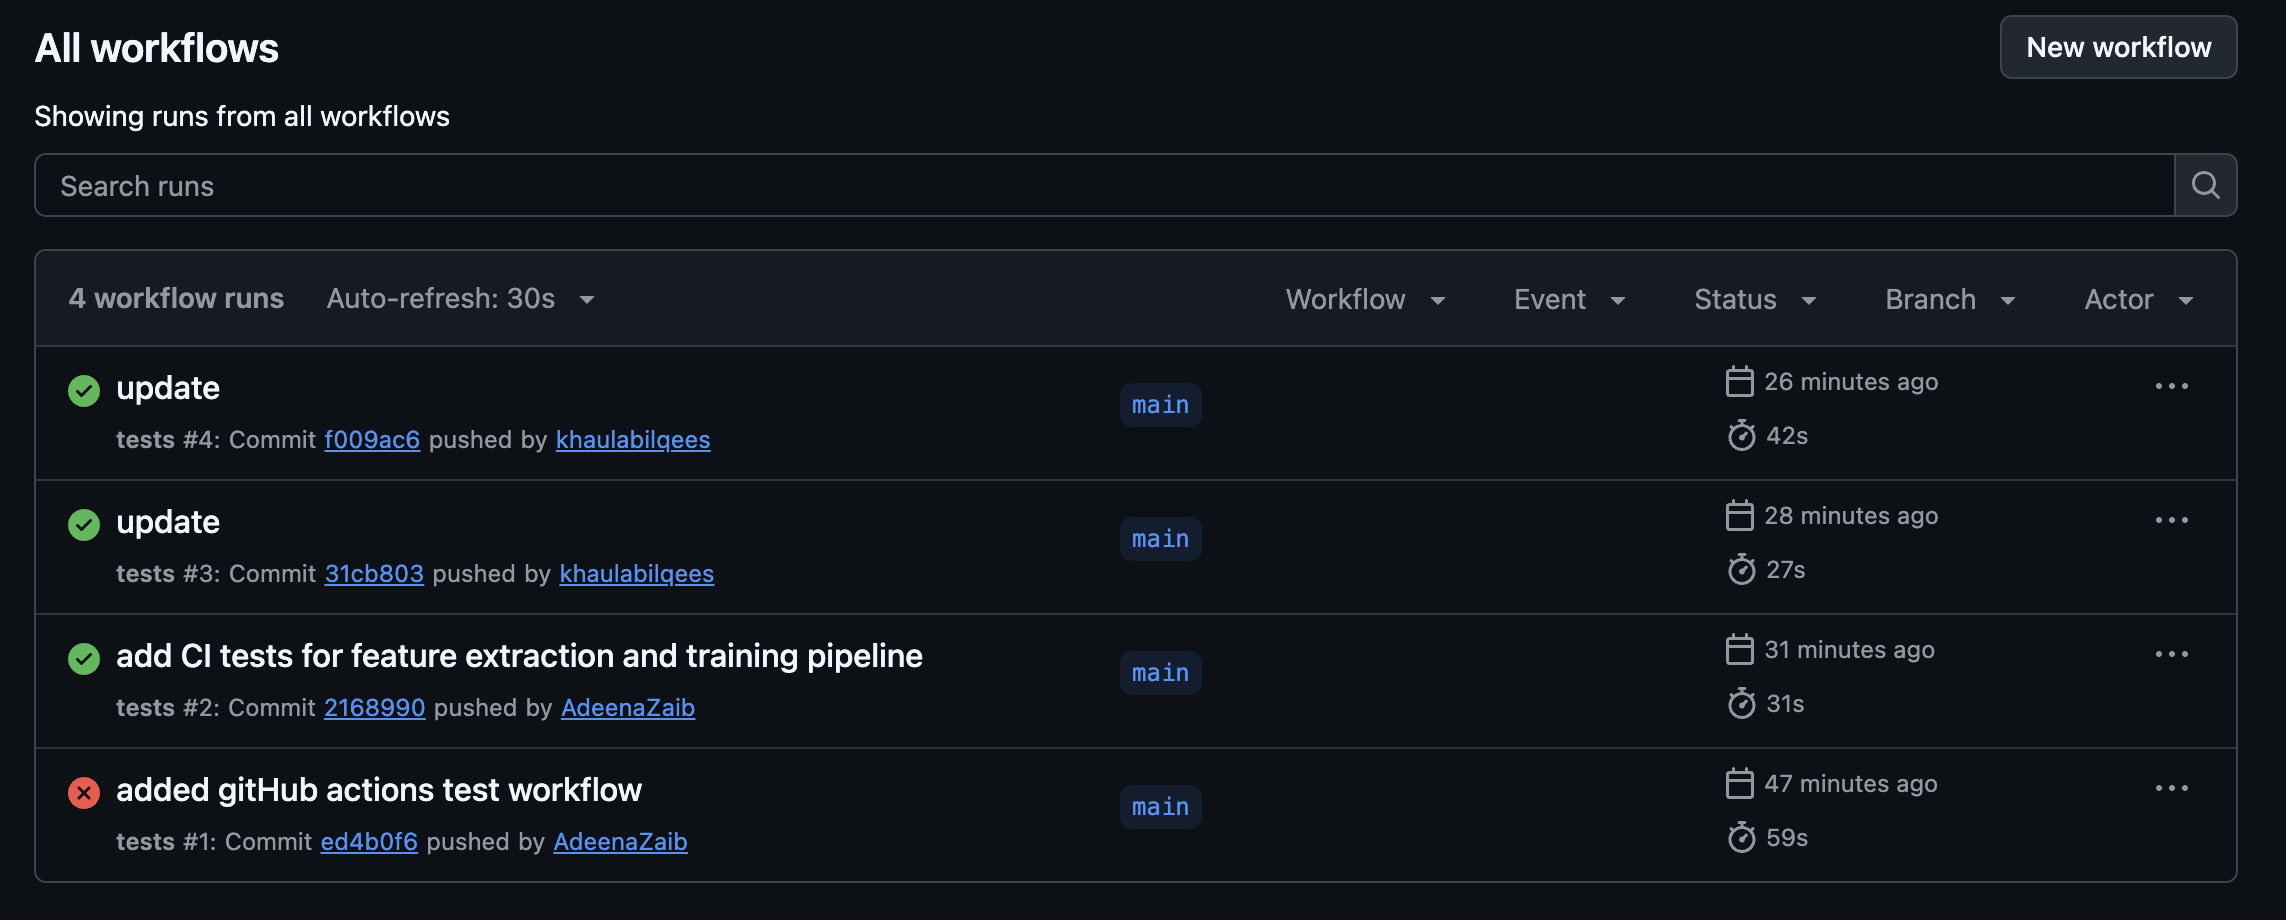
\includegraphics[width=0.95\textwidth]{workflow.png}
\caption[GitHub Actions run history]{GitHub Actions run history. Each run is tied to a commit and to the member
who pushed it, which is the per-member development evidence this section reports.
Run \#1 failed and the following runs pass, which records a real correction rather
than a repository created immediately before submission.}
\label{fig:ci}
\end{figure}

Two properties of this history are worth stating explicitly, because they are what
the evidence is for. First, the pushes are distributed across both members:
runs \#1 and \#2 were pushed by the first member and runs \#3 and \#4 by the
second, so the contribution record is visible in the tooling rather than asserted in
this document. Second, the first run failed and subsequent runs pass. That sequence
is retained deliberately: it shows the pipeline being established and corrected during
the reporting period.

\section{Milestones and Commit Evidence}
The automated suite is itself the milestone evidence for modules M2 and M3. It
contains fourteen tests, of which three are dataset invariants that run only when
\texttt{features.csv} is present and are therefore exercising the real extracted
dataset rather than synthetic fixtures. Three of those tests encode the corrections
recorded as defects in Section~\ref{sec:defects}: that attack labels are confined to the target
zone (DEF-01), that the cross-zone residual is not identically zero, and that the
victim zone rotates across runs so that the detector cannot memorise a single zone.

\begin{longtable}{p{0.14\textwidth} p{0.30\textwidth} p{0.46\textwidth}}
\caption{Milestones against the commits that completed them}\label{tab:milestones}\\
\toprule
\textbf{Commit} & \textbf{Milestone} & \textbf{Module and evidence} \\
\midrule
\endfirsthead
\toprule
\textbf{Commit} & \textbf{Milestone} & \textbf{Module and evidence} \\
\midrule
\endhead
\texttt{0506e63} & Proof of concept & Pre-proposal demonstrator \\
\addlinespace
\texttt{8b765f6} & M1 complete: zonal topology simulated &
\texttt{CarazoneZonalNetwork.ned}; Figure~\ref{fig:topology} \\
\addlinespace
\texttt{856beba} & M3 complete: feature extraction, including the cross-zone residual &
\texttt{extract\_features.py}; ablation in Section~\ref{sec:acceptance-validation} \\
\addlinespace
\texttt{ed4b0f6} & Continuous integration established &
First workflow run; failed, and corrected in the next commit \\
\addlinespace
\texttt{2168990} & Automated test suite covering M2 and M3 &
Fourteen tests; three encode the DEF-01 correction (Appendix~\ref{app:test-cases}) \\
\addlinespace
\texttt{31cb803}, \texttt{f009ac6} & Topology and configuration revisions &
Passing workflow runs \#3 and \#4 \\
\bottomrule
\end{longtable}

\section{Tools and Tool-Assisted Development}

\begin{longtable}{p{0.24\textwidth} p{0.3\textwidth} p{0.38\textwidth}}
\caption{Tool and AI-assistance disclosure}\\
\toprule
\textbf{Tool} & \textbf{Used for} & \textbf{Boundary} \\
\midrule
\endfirsthead
\toprule
\textbf{Tool} & \textbf{Used for} & \textbf{Boundary} \\
\midrule
\endhead
OMNeT++ / INET & Simulation framework & Standard open-source components used as
published; the topology, scenario configurations and attack injection logic are the
team's own work \\
\addlinespace
Generative AI assistants & Literature search support, document drafting, code
scaffolding, report structuring and review &
Core detection model design, federated architecture decisions, attack
implementation, simulation configuration, experimental results and their
interpretation are the team's own work. Generated text has been reviewed, verified
against primary sources and rewritten by the authors. No reported result is AI
generated. \\
\bottomrule
\end{longtable}

% [[VERIFY]] Extend this to the exact level of disclosure your department requires,
% and ensure both members can explain any section they did not personally draft.

\section{External Components and Dependencies}
\label{sec:dependencies}

\begin{longtable}{p{0.2\textwidth} p{0.14\textwidth} p{0.2\textwidth} p{0.36\textwidth}}
\toprule
\textbf{Component} & \textbf{Version} & \textbf{Licence} & \textbf{Use} \\
\midrule
\endhead
OMNeT++ & 6.4.0 & Academic Public License & Simulation kernel \\
INET & 4.7.0 & LGPL & TSN, gPTP, clock models \\
Python & 3.x & PSF & Extraction, training \\
Flower & not yet adopted & Apache 2.0 & Federated learning framework; selected for Iteration~03, not yet introduced into the build \\
\bottomrule
\end{longtable}

\section{Risks and Mitigation}

\begin{longtable}{p{0.24\textwidth} p{0.1\textwidth} p{0.28\textwidth} p{0.28\textwidth}}
\caption{Risk register}\\
\toprule
\textbf{Risk} & \textbf{L\,/\,I} & \textbf{Mitigation} & \textbf{Trigger / fallback} \\
\midrule
\endfirsthead
\toprule
\textbf{Risk} & \textbf{L\,/\,I} & \textbf{Mitigation} & \textbf{Trigger / fallback} \\
\midrule
\endhead
Protocol-native features do not outperform generic traffic features &
Med / High &
Run the controlled comparison centrally and early, before federated infrastructure is
built &
If no advantage is demonstrated, report the negative result and reposition the
contribution around federated zone-level detection and attribution \\
\addlinespace
Required internal protocol state is not exposed by the simulation framework &
Med / High &
Verify observability per feature before committing the feature &
Substitute an observable proxy or instrument the module explicitly \\
\addlinespace
FedAvg does not outperform local-only training under non-IID zones &
Med / Med &
Introduce genuine zone heterogeneity; normalise features; report worst-client
performance &
Report as a legitimate finding; FedProx retained as an extension, not a rescue \\
\addlinespace
Feature leakage through adjacent-window splitting &
Med / High &
Split by run and seed, never by window (integrity rule R3) &
Rebuild the dataset and record the change \\
\addlinespace
Scope expansion through additional attacks or models &
High / High &
Protect committed scope; extensions gated on completion of the core path &
Drop schedule-window detection, FedProx and conformal calibration first, in that
order; reduce FRER to a single redundant stream pair before dropping it \\
\addlinespace
Remaining implementation compressed into FYP-2 &
High / High &
Sequence the decision gate first so that a null result is found early &
Reduce to a single attack class with full evaluation rather than several partially
evaluated \\
\bottomrule
\end{longtable}

\section{Security and Privacy Considerations}
All data is synthetic. No personal, vehicle or OEM data is processed. The federated
design transmits model parameters only; raw feature records never leave the client
(NFR-07), which is verified by the acceptance check on FR-13. Attack implementations
are confined to the simulation environment. Secure aggregation, differential privacy
and model-poisoning resistance are outside committed scope and are stated as
limitations rather than claimed properties.

\section{Current Limitations}
\label{sec:limitations}
\begin{enumerate}
  \item Detection results are centralized only; no federated result is claimed.
  \item Zones are currently symmetric, so federated behaviour cannot yet be assessed.
  \item The injected attack is large relative to the benign steady-state envelope; the
        intensity at which detection degrades has not been established.
  \item Oscillator drift manipulation is not realisable as a runtime attack under the
        current framework, reducing the committed attack set to two classes.
  \item Time-aware shaping is not configured, so schedule-conformance features and
        deadline-miss consequences are unavailable.
  \item The approach is insensitive to grandmaster-level compromise by construction.
  \item The static-environment assumption (A1) excludes networks that reconfigure at
        runtime.
  \item Evaluation is simulation-only; attacks are synthetic and no hardware
        validation is performed.
  \item The alert surface is a presentation mock-up and is not yet driven by model
        output.
\end{enumerate}

% ============================================================